\documentclass[border=20pt]{standalone}
\usepackage{tikz}
\usetikzlibrary{positioning, arrows.meta, fit, backgrounds, calc, decorations.pathreplacing}
\usepackage{amsmath, amssymb}
\usepackage[T1]{fontenc}
\usepackage{lmodern}

\definecolor{embedcolor}{HTML}{4A90D9}
\definecolor{attncolor}{HTML}{E8734A}
\definecolor{mlpcolor}{HTML}{5CB85C}
\definecolor{normcolor}{HTML}{F5C242}
\definecolor{outcolor}{HTML}{9B59B6}
\definecolor{bgblock}{HTML}{F7F7F7}
\definecolor{arrow}{HTML}{333333}
\definecolor{scalebg}{HTML}{EEF4FF}

\begin{document}
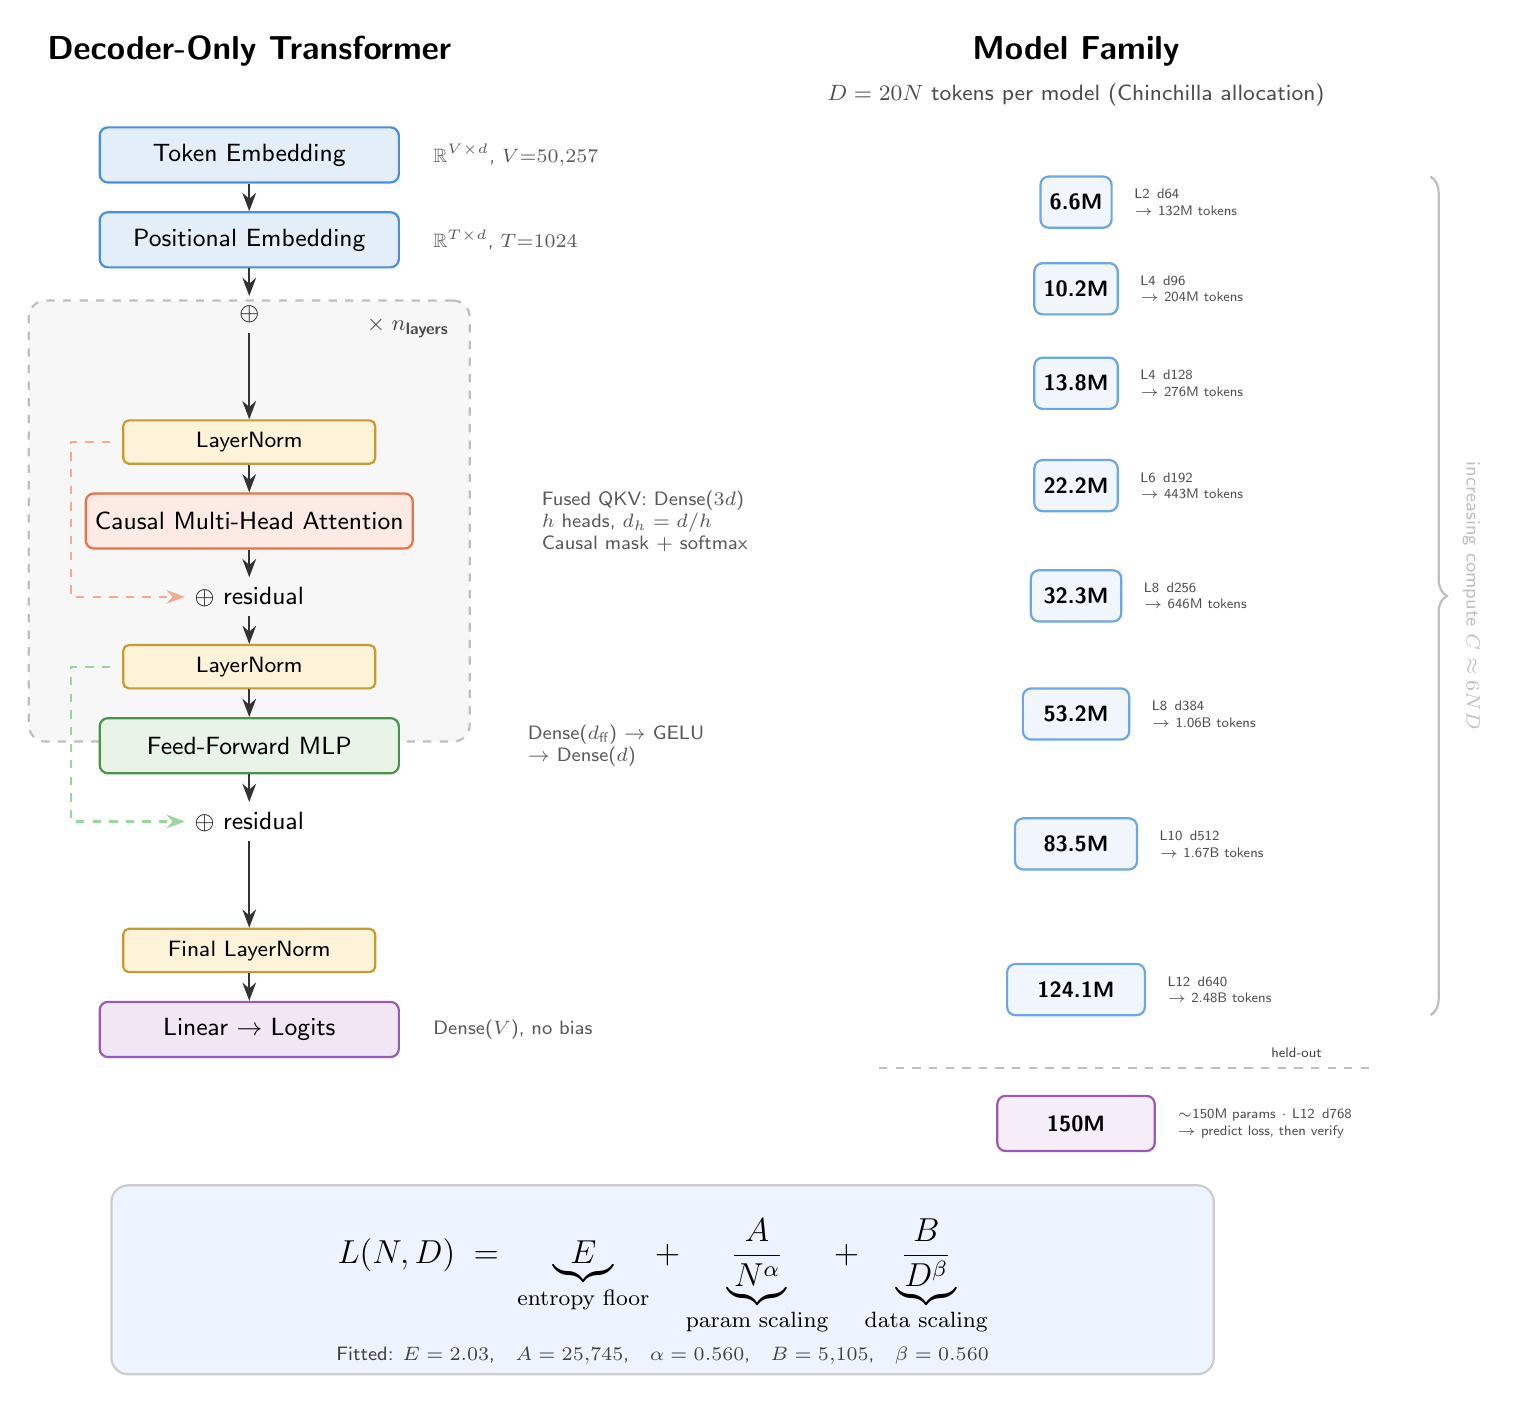
\begin{tikzpicture}[
    >=Stealth,
    node distance=0.6cm,
    every node/.style={font=\sffamily\small},
    block/.style={draw, rounded corners=3pt, minimum width=3.8cm, minimum height=0.7cm, align=center, thick},
    smallblock/.style={draw, rounded corners=2pt, minimum width=3.2cm, minimum height=0.55cm, align=center, thick, font=\sffamily\footnotesize},
    label/.style={font=\sffamily\scriptsize\color{gray!70!black}, align=left},
]

% ============================================================
% LEFT: Transformer Architecture
% ============================================================

\node[font=\sffamily\large\bfseries, anchor=south] at (0, 11.8) {Decoder-Only Transformer};

% Input
\node[block, fill=embedcolor!15, draw=embedcolor] (tokem) at (0, 10.8) {Token Embedding};
\node[label, right=0.3cm of tokem] {$\mathbb{R}^{V \times d}$, $V{=}50{,}257$};

\node[block, fill=embedcolor!15, draw=embedcolor, below=0.35cm of tokem] (posem) {Positional Embedding};
\node[label, right=0.3cm of posem] {$\mathbb{R}^{T \times d}$, $T{=}1024$};

\node[below=0.35cm of posem, font=\sffamily\small] (plus) {$\oplus$};

% Transformer block background
\begin{scope}[on background layer]
    \node[draw=gray!50, rounded corners=6pt, fill=bgblock, thick, dashed,
          minimum width=5.6cm, minimum height=5.6cm] (blockbg) at (0, 6.15) {};
\end{scope}

\node[font=\sffamily\footnotesize\bfseries\color{gray!60!black}, anchor=north east] at ($(blockbg.north east)+(-0.15,-0.1)$) {$\times\; n_{\text{layers}}$};

% Layer Norm 1
\node[smallblock, fill=normcolor!20, draw=normcolor!80!black, below=1.1cm of plus] (ln1) {LayerNorm};

% Causal MHA
\node[block, fill=attncolor!15, draw=attncolor, below=0.35cm of ln1] (attn) {Causal Multi-Head Attention};
\node[label, right=1.5cm of attn.east, text width=3.5cm] (attnlabel) {Fused QKV: Dense($3d$)\\$h$ heads, $d_h = d/h$\\Causal mask $+ $ softmax};

% Residual 1
\node[below=0.35cm of attn, font=\sffamily\small] (res1) {$\oplus$ residual};

% Layer Norm 2
\node[smallblock, fill=normcolor!20, draw=normcolor!80!black, below=0.35cm of res1] (ln2) {LayerNorm};

% MLP
\node[block, fill=mlpcolor!15, draw=mlpcolor!80!black, below=0.35cm of ln2] (mlp) {Feed-Forward MLP};
\node[label, right=1.5cm of mlp.east, text width=3cm] {Dense($d_{\text{ff}}$) $\to$ GELU\\$\to$ Dense($d$)};

% Residual 2
\node[below=0.35cm of mlp, font=\sffamily\small] (res2) {$\oplus$ residual};

% Final LN
\node[smallblock, fill=normcolor!20, draw=normcolor!80!black, below=1.1cm of res2] (lnf) {Final LayerNorm};

% Output projection
\node[block, fill=outcolor!15, draw=outcolor, below=0.35cm of lnf] (out) {Linear $\to$ Logits};
\node[label, right=0.3cm of out] {Dense($V$), no bias};

% Arrows
\draw[->, thick, color=arrow] (tokem) -- (posem);
\draw[->, thick, color=arrow] (posem) -- (plus);
\draw[->, thick, color=arrow] (plus) -- (ln1);
\draw[->, thick, color=arrow] (ln1) -- (attn);
\draw[->, thick, color=arrow] (attn) -- (res1);
\draw[->, thick, color=arrow] (res1) -- (ln2);
\draw[->, thick, color=arrow] (ln2) -- (mlp);
\draw[->, thick, color=arrow] (mlp) -- (res2);
\draw[->, thick, color=arrow] (res2) -- (lnf);
\draw[->, thick, color=arrow] (lnf) -- (out);

% Residual bypass arrows
\draw[->, thick, color=attncolor!60, dashed] ($(ln1.west)+(-0.15,0)$) -- +(-0.5,0) |- (res1.west);
\draw[->, thick, color=mlpcolor!60, dashed] ($(ln2.west)+(-0.15,0)$) -- +(-0.5,0) |- (res2.west);

% ============================================================
% RIGHT: Model Family Scaling Diagram
% ============================================================

\begin{scope}[xshift=10.5cm]

\node[font=\sffamily\large\bfseries, anchor=south] at (0, 11.8) {Model Family};
\node[font=\sffamily\footnotesize\color{gray!60!black}, anchor=south] at (0, 11.3) {$D = 20N$ tokens per model (Chinchilla allocation)};

% Scaling boxes — increasing size represents increasing model size
% Each box: model name, params, key dims

\foreach \i/\name/\dims/\tok/\w/\y in {
    0/6.6M/{L2\, d64}/132M/0.55/10.2,
    1/10.2M/{L4\, d96}/204M/0.7/9.1,
    2/13.8M/{L4\, d128}/276M/0.85/7.9,
    3/22.2M/{L6\, d192}/443M/1.0/6.6,
    4/32.3M/{L8\, d256}/646M/1.15/5.2,
    5/53.2M/{L8\, d384}/1.06B/1.35/3.7,
    6/83.5M/{L10\, d512}/1.67B/1.55/2.05,
    7/124.1M/{L12\, d640}/2.48B/1.75/0.2%
}{
    \node[draw=embedcolor!80, fill=embedcolor!8, rounded corners=3pt,
          minimum width=\w cm, minimum height=0.65cm, thick,
          font=\sffamily\footnotesize\bfseries] (m\i) at (0, \y) {\name};
    \node[font=\sffamily\tiny\color{gray!60!black}, right=0.15cm of m\i.east, anchor=west, text width=3.2cm]
         {\dims\\$\to$ \tok\ tokens};
}

% Held-out model (visually separated)
\draw[dashed, gray!50, thick] (-2.5, -0.8) -- (3.8, -0.8);
\node[font=\sffamily\tiny\color{gray!50!black}] at (2.8, -0.6) {held-out};

\node[draw=outcolor, fill=outcolor!10, rounded corners=3pt,
      minimum width=2.0cm, minimum height=0.7cm, thick,
      font=\sffamily\footnotesize\bfseries] (mheld) at (0, -1.5) {150M};
\node[font=\sffamily\tiny\color{gray!60!black}, right=0.15cm of mheld.east, anchor=west, text width=3.2cm]
     {$\sim$150M params $\cdot$ L12\, d768\\$\to$ predict loss, then verify};

% Arrow showing scaling direction
\draw[decorate, decoration={brace, amplitude=6pt, mirror}, thick, gray!50]
    (4.5, 0.2 - 0.325) -- (4.5, 10.2 + 0.325)
    node[midway, right=8pt, font=\sffamily\scriptsize\color{gray!60!black}, rotate=270, anchor=south] {increasing compute $C \approx 6ND$};

\end{scope}

% ============================================================
% BOTTOM: Scaling Law Equation
% ============================================================

\node[draw=gray!40, rounded corners=6pt, fill=scalebg, thick,
      minimum width=14cm, minimum height=2.4cm, anchor=south] (eqbox) at (5.25, -4.7) {};

\node[font=\large, anchor=center] at (5.25, -3.45) {
    $L(N, D) \;=\; \underbrace{E}_{\text{entropy floor}} + \underbrace{\frac{A}{N^{\alpha}}}_{\text{param scaling}} + \underbrace{\frac{B}{D^{\beta}}}_{\text{data scaling}}$
};

\node[font=\sffamily\scriptsize\color{gray!50!black}, anchor=center] at (5.25, -4.45) {
    Fitted: $E = 2.03$,\quad $A = 25{,}745$,\quad $\alpha = 0.560$,\quad $B = 5{,}105$,\quad $\beta = 0.560$
};

\end{tikzpicture}
\end{document}
